
\documentclass[tikz,border=5pt]{standalone}

% Core packages
\usepackage{amsmath,amssymb}
\usepackage{tikz}
\usepackage{tikz-cd}
\usepackage{pgfplots}
\usepackage{multicol}
\usepackage{xcolor}
\usepackage{caption}
\usepackage{float}
\usepackage{kotex}

% TikZ / PGF configuration
\usetikzlibrary{
  arrows.meta,
  calc,
  positioning,
  shapes.geometric,
  shapes.symbols,
  fit,
  backgrounds,
  patterns,
  matrix,
  intersections,
  decorations.pathmorphing,
  decorations.markings,
  angles,
  quotes
}
\pgfplotsset{compat=1.18}

% Reusable TikZ styles
\tikzset{
  >=stealth,
  line cap=round,
  line join=round,
  every picture/.style={line width=0.9pt},
  box/.style={draw, rounded corners, minimum width=2.8cm, minimum height=1.2cm, align=center},
  circlebox/.style={draw, circle, minimum size=1cm, align=center},
  arrow/.style={->, thick},
  dashedarrow/.style={->, thick, dashed},
  point/.style={circle, fill, inner sep=1.2pt},
  gridhelp/.style={help lines, gray!35},
  highlight/.style={fill=blue!10, draw=blue!60!black},
  3D/.style={
    x={(-0.60cm,-0.42cm)},
    y={(0.78cm,0cm)},
    z={(0cm,0.78cm)}
  }
}


\begin{document}

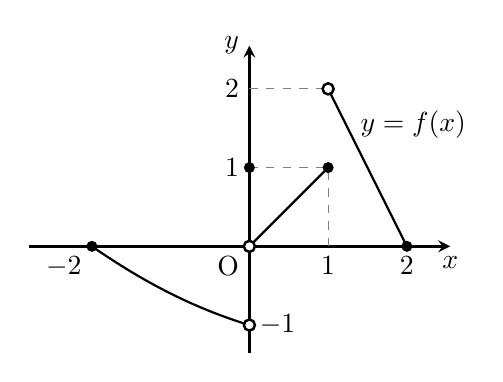
\begin{tikzpicture}

% 좌표축
\draw[-stealth] (-2.8,0) -- (2.55,0) node[below] {$x$};
\draw[-stealth] (0,-1.35) -- (0,2.55) node[left] {$y$};

% 보조 점선
\draw[dashed, thin, gray] (0,2) -- (1,2);
\draw[dashed, thin, gray] (0,1) -- (1,1);
\draw[dashed, thin, gray] (1,0) -- (1,1);

% 함수 그래프
\draw[thick] (-2,0) .. controls (-1.35,-0.45) and (-0.72,-0.78) .. (0,-1);
\draw[thick] (0,0) -- (1,1);
\draw[thick] (1,2) -- (2,0);

% 축 레이블
\fill (-2,0) circle (2pt) node[below left] at (-2,0) {$-2$};
\node[below] at (1,0) {$1$};
\node[below] at (2,0) {$2$};
\node[below left] at (0,0) {$\mathrm{O}$};
\fill (0,1) circle (2pt) node[left] at (0,2) {$2$};
\filldraw[fill=white,draw=black] (0,-1) circle (2pt) node[right] at (0,-1) {$-1$};
\node[left] at (0,1) {$1$};
\filldraw[fill=white,draw=black] (1,2) circle (2pt);
\filldraw[fill=white,draw=black] (0,0) circle (2pt);
\fill (1,1) circle (2pt);
\fill (2,0) circle (2pt);

% 함수 레이블
\node[right] at (1.28,1.55) {$y=f(x)$};
 
\end{tikzpicture}

\end{document}

